% Options for packages loaded elsewhere
\PassOptionsToPackage{unicode}{hyperref}
\PassOptionsToPackage{hyphens}{url}
%
\documentclass[
]{article}
\usepackage{amsmath,amssymb}
\usepackage{lmodern}
\usepackage{iftex}
\ifPDFTeX
  \usepackage[T1]{fontenc}
  \usepackage[utf8]{inputenc}
  \usepackage{textcomp} % provide euro and other symbols
\else % if luatex or xetex
  \usepackage{unicode-math}
  \defaultfontfeatures{Scale=MatchLowercase}
  \defaultfontfeatures[\rmfamily]{Ligatures=TeX,Scale=1}
\fi
% Use upquote if available, for straight quotes in verbatim environments
\IfFileExists{upquote.sty}{\usepackage{upquote}}{}
\IfFileExists{microtype.sty}{% use microtype if available
  \usepackage[]{microtype}
  \UseMicrotypeSet[protrusion]{basicmath} % disable protrusion for tt fonts
}{}
\makeatletter
\@ifundefined{KOMAClassName}{% if non-KOMA class
  \IfFileExists{parskip.sty}{%
    \usepackage{parskip}
  }{% else
    \setlength{\parindent}{0pt}
    \setlength{\parskip}{6pt plus 2pt minus 1pt}}
}{% if KOMA class
  \KOMAoptions{parskip=half}}
\makeatother
\usepackage{xcolor}
\usepackage[margin=1in]{geometry}
\usepackage{color}
\usepackage{fancyvrb}
\newcommand{\VerbBar}{|}
\newcommand{\VERB}{\Verb[commandchars=\\\{\}]}
\DefineVerbatimEnvironment{Highlighting}{Verbatim}{commandchars=\\\{\}}
% Add ',fontsize=\small' for more characters per line
\usepackage{framed}
\definecolor{shadecolor}{RGB}{248,248,248}
\newenvironment{Shaded}{\begin{snugshade}}{\end{snugshade}}
\newcommand{\AlertTok}[1]{\textcolor[rgb]{0.94,0.16,0.16}{#1}}
\newcommand{\AnnotationTok}[1]{\textcolor[rgb]{0.56,0.35,0.01}{\textbf{\textit{#1}}}}
\newcommand{\AttributeTok}[1]{\textcolor[rgb]{0.77,0.63,0.00}{#1}}
\newcommand{\BaseNTok}[1]{\textcolor[rgb]{0.00,0.00,0.81}{#1}}
\newcommand{\BuiltInTok}[1]{#1}
\newcommand{\CharTok}[1]{\textcolor[rgb]{0.31,0.60,0.02}{#1}}
\newcommand{\CommentTok}[1]{\textcolor[rgb]{0.56,0.35,0.01}{\textit{#1}}}
\newcommand{\CommentVarTok}[1]{\textcolor[rgb]{0.56,0.35,0.01}{\textbf{\textit{#1}}}}
\newcommand{\ConstantTok}[1]{\textcolor[rgb]{0.00,0.00,0.00}{#1}}
\newcommand{\ControlFlowTok}[1]{\textcolor[rgb]{0.13,0.29,0.53}{\textbf{#1}}}
\newcommand{\DataTypeTok}[1]{\textcolor[rgb]{0.13,0.29,0.53}{#1}}
\newcommand{\DecValTok}[1]{\textcolor[rgb]{0.00,0.00,0.81}{#1}}
\newcommand{\DocumentationTok}[1]{\textcolor[rgb]{0.56,0.35,0.01}{\textbf{\textit{#1}}}}
\newcommand{\ErrorTok}[1]{\textcolor[rgb]{0.64,0.00,0.00}{\textbf{#1}}}
\newcommand{\ExtensionTok}[1]{#1}
\newcommand{\FloatTok}[1]{\textcolor[rgb]{0.00,0.00,0.81}{#1}}
\newcommand{\FunctionTok}[1]{\textcolor[rgb]{0.00,0.00,0.00}{#1}}
\newcommand{\ImportTok}[1]{#1}
\newcommand{\InformationTok}[1]{\textcolor[rgb]{0.56,0.35,0.01}{\textbf{\textit{#1}}}}
\newcommand{\KeywordTok}[1]{\textcolor[rgb]{0.13,0.29,0.53}{\textbf{#1}}}
\newcommand{\NormalTok}[1]{#1}
\newcommand{\OperatorTok}[1]{\textcolor[rgb]{0.81,0.36,0.00}{\textbf{#1}}}
\newcommand{\OtherTok}[1]{\textcolor[rgb]{0.56,0.35,0.01}{#1}}
\newcommand{\PreprocessorTok}[1]{\textcolor[rgb]{0.56,0.35,0.01}{\textit{#1}}}
\newcommand{\RegionMarkerTok}[1]{#1}
\newcommand{\SpecialCharTok}[1]{\textcolor[rgb]{0.00,0.00,0.00}{#1}}
\newcommand{\SpecialStringTok}[1]{\textcolor[rgb]{0.31,0.60,0.02}{#1}}
\newcommand{\StringTok}[1]{\textcolor[rgb]{0.31,0.60,0.02}{#1}}
\newcommand{\VariableTok}[1]{\textcolor[rgb]{0.00,0.00,0.00}{#1}}
\newcommand{\VerbatimStringTok}[1]{\textcolor[rgb]{0.31,0.60,0.02}{#1}}
\newcommand{\WarningTok}[1]{\textcolor[rgb]{0.56,0.35,0.01}{\textbf{\textit{#1}}}}
\usepackage{graphicx}
\makeatletter
\def\maxwidth{\ifdim\Gin@nat@width>\linewidth\linewidth\else\Gin@nat@width\fi}
\def\maxheight{\ifdim\Gin@nat@height>\textheight\textheight\else\Gin@nat@height\fi}
\makeatother
% Scale images if necessary, so that they will not overflow the page
% margins by default, and it is still possible to overwrite the defaults
% using explicit options in \includegraphics[width, height, ...]{}
\setkeys{Gin}{width=\maxwidth,height=\maxheight,keepaspectratio}
% Set default figure placement to htbp
\makeatletter
\def\fps@figure{htbp}
\makeatother
\setlength{\emergencystretch}{3em} % prevent overfull lines
\providecommand{\tightlist}{%
  \setlength{\itemsep}{0pt}\setlength{\parskip}{0pt}}
\setcounter{secnumdepth}{-\maxdimen} % remove section numbering
\usepackage{booktabs}
\usepackage{longtable}
\usepackage{array}
\usepackage{multirow}
\usepackage{wrapfig}
\usepackage{float}
\usepackage{colortbl}
\usepackage{pdflscape}
\usepackage{tabu}
\usepackage{threeparttable}
\usepackage{threeparttablex}
\usepackage[normalem]{ulem}
\usepackage{makecell}
\usepackage{xcolor}
\ifLuaTeX
  \usepackage{selnolig}  % disable illegal ligatures
\fi
\IfFileExists{bookmark.sty}{\usepackage{bookmark}}{\usepackage{hyperref}}
\IfFileExists{xurl.sty}{\usepackage{xurl}}{} % add URL line breaks if available
\urlstyle{same} % disable monospaced font for URLs
\hypersetup{
  pdftitle={Appendix: Source code},
  hidelinks,
  pdfcreator={LaTeX via pandoc}}

\title{Appendix: Source code}
\author{}
\date{\vspace{-2.5em}2024-04-21}

\begin{document}
\maketitle

\begin{Shaded}
\begin{Highlighting}[]
\NormalTok{knitr}\SpecialCharTok{::}\NormalTok{opts\_chunk}\SpecialCharTok{$}\FunctionTok{set}\NormalTok{(}\AttributeTok{echo =} \ConstantTok{TRUE}\NormalTok{)}
\FunctionTok{rm}\NormalTok{(}\AttributeTok{list =} \FunctionTok{ls}\NormalTok{())}
\FunctionTok{gc}\NormalTok{()}
\end{Highlighting}
\end{Shaded}

\begin{verbatim}
##          used (Mb) gc trigger (Mb) max used (Mb)
## Ncells 476581 25.5    1029462   55   664394 35.5
## Vcells 894613  6.9    8388608   64  1814579 13.9
\end{verbatim}

\begin{Shaded}
\begin{Highlighting}[]
\FunctionTok{set.seed}\NormalTok{(}\DecValTok{1}\NormalTok{)}
\FunctionTok{options}\NormalTok{(}\AttributeTok{digits=}\DecValTok{6}\NormalTok{) }
\ControlFlowTok{if}\NormalTok{ (}\SpecialCharTok{!}\FunctionTok{require}\NormalTok{(}\StringTok{"pacman"}\NormalTok{)) }\FunctionTok{install.packages}\NormalTok{(}\StringTok{"pacman"}\NormalTok{)}
\end{Highlighting}
\end{Shaded}

\begin{verbatim}
## Loading required package: pacman
\end{verbatim}

\begin{Shaded}
\begin{Highlighting}[]
\NormalTok{pacman}\SpecialCharTok{::}\FunctionTok{p\_load}\NormalTok{(}
\NormalTok{  plm,}
\NormalTok{  ggplot2,}
\NormalTok{  tidyverse,}
\NormalTok{  fixest,}
\NormalTok{  knitr,}
\NormalTok{  kableExtra,}
\NormalTok{  tidymodels,}
\NormalTok{  modelsummary,}
\NormalTok{  ggplot2}
\NormalTok{)}
\end{Highlighting}
\end{Shaded}

\hypertarget{data}{%
\subsubsection{Data}\label{data}}

\begin{Shaded}
\begin{Highlighting}[]
\NormalTok{df }\OtherTok{\textless{}{-}} \FunctionTok{read\_csv}\NormalTok{(}\StringTok{"./input/MROZ\_mini.csv"}\NormalTok{)}
\end{Highlighting}
\end{Shaded}

\begin{verbatim}
## Rows: 428 Columns: 3
## -- Column specification --------------------------------------------------------
## Delimiter: ","
## dbl (3): educ, fatheduc, lwage
## 
## i Use `spec()` to retrieve the full column specification for this data.
## i Specify the column types or set `show_col_types = FALSE` to quiet this message.
\end{verbatim}

\begin{Shaded}
\begin{Highlighting}[]
\FunctionTok{head}\NormalTok{(df, }\DecValTok{30}\NormalTok{)}
\end{Highlighting}
\end{Shaded}

\begin{verbatim}
## # A tibble: 30 x 3
##     educ fatheduc  lwage
##    <dbl>    <dbl>  <dbl>
##  1    12        7 1.21  
##  2    12        7 0.329 
##  3    12        7 1.51  
##  4    12        7 0.0921
##  5    14       14 1.52  
##  6    12        7 1.56  
##  7    16        7 2.12  
##  8    12        3 2.06  
##  9    12        7 0.754 
## 10    12        7 1.54  
## # i 20 more rows
\end{verbatim}

\hypertarget{question-1-1}{%
\section{Question 1-1}\label{question-1-1}}

\begin{Shaded}
\begin{Highlighting}[]
\DocumentationTok{\#\#\#\#\# Question 1 \#\#\#\#\#}

\NormalTok{const }\OtherTok{\textless{}{-}} \FunctionTok{rep}\NormalTok{(}\DecValTok{1}\NormalTok{, }\FunctionTok{nrow}\NormalTok{(df))}
\NormalTok{Mat\_X }\OtherTok{\textless{}{-}} \FunctionTok{as.matrix}\NormalTok{(}\FunctionTok{cbind}\NormalTok{(const, df[, }\DecValTok{1}\NormalTok{]))}
\NormalTok{Mat\_y }\OtherTok{\textless{}{-}} \FunctionTok{as.matrix}\NormalTok{(df[, }\DecValTok{3}\NormalTok{])}

\CommentTok{\# Computing beta\_hat}
\NormalTok{analytical\_beta }\OtherTok{\textless{}{-}} \FunctionTok{solve}\NormalTok{(}\FunctionTok{t}\NormalTok{(Mat\_X) }\SpecialCharTok{\%*\%}\NormalTok{ Mat\_X) }\SpecialCharTok{\%*\%}\NormalTok{ (}\FunctionTok{t}\NormalTok{(Mat\_X) }\SpecialCharTok{\%*\%}\NormalTok{ Mat\_y) }
\end{Highlighting}
\end{Shaded}

\hypertarget{answer-to-q1-1}{%
\subsection{Answer to Q1-1}\label{answer-to-q1-1}}

\begin{Shaded}
\begin{Highlighting}[]
\DocumentationTok{\#\#\# Q1 Answer }\AlertTok{\#\#\#}
\FunctionTok{print}\NormalTok{(}\FunctionTok{paste}\NormalTok{(}\StringTok{"beta\_0: "}\NormalTok{, analytical\_beta[}\DecValTok{1}\NormalTok{]))}
\end{Highlighting}
\end{Shaded}

\begin{verbatim}
## [1] "beta_0:  -0.185196923871551"
\end{verbatim}

\begin{Shaded}
\begin{Highlighting}[]
\FunctionTok{print}\NormalTok{(}\FunctionTok{paste}\NormalTok{(}\StringTok{"beta\_1: "}\NormalTok{, analytical\_beta[}\DecValTok{2}\NormalTok{]))}
\end{Highlighting}
\end{Shaded}

\begin{verbatim}
## [1] "beta_1:  0.108648664436512"
\end{verbatim}

\hypertarget{result-table-in-q1-1}{%
\subsection{Result table in Q1-1}\label{result-table-in-q1-1}}

\begin{Shaded}
\begin{Highlighting}[]
\CommentTok{\# Create the result table}
\NormalTok{coefs\_Q1\_1 }\OtherTok{\textless{}{-}} \FunctionTok{data.frame}\NormalTok{(}
  \AttributeTok{variable =} \FunctionTok{c}\NormalTok{(}\StringTok{"Constant"}\NormalTok{,  }\StringTok{"educ"}\NormalTok{, }\StringTok{"Num.Obs."}\NormalTok{),}
  \AttributeTok{OLS\_model =} \FunctionTok{c}\NormalTok{(}\FunctionTok{format}\NormalTok{(analytical\_beta[}\DecValTok{1}\NormalTok{], }\AttributeTok{digits =} \DecValTok{6}\NormalTok{),}
               \FunctionTok{format}\NormalTok{(analytical\_beta[}\DecValTok{2}\NormalTok{], }\AttributeTok{digits =} \DecValTok{6}\NormalTok{),}
               \FunctionTok{format}\NormalTok{(}\FunctionTok{nrow}\NormalTok{(df), }\AttributeTok{digits =} \DecValTok{1}\NormalTok{))}
\NormalTok{)}

\CommentTok{\# result the table}
\NormalTok{coefs\_table\_Q1\_1  }\OtherTok{\textless{}{-}} \FunctionTok{kable}\NormalTok{(coefs\_Q1\_1, }
                           \AttributeTok{caption =} \StringTok{"Analytical OLS estimation Result"}\NormalTok{,}
                           \AttributeTok{align =} \FunctionTok{c}\NormalTok{(}\StringTok{"l"}\NormalTok{, }\StringTok{"c"}\NormalTok{))  }\SpecialCharTok{\%\textgreater{}\%}
  \FunctionTok{kable\_styling}\NormalTok{(}\AttributeTok{full\_width =} \ConstantTok{FALSE}\NormalTok{) }
\NormalTok{coefs\_table\_Q1\_1 }
\end{Highlighting}
\end{Shaded}

\begin{longtable}[t]{lc}
\caption{\label{tab:unnamed-chunk-4}Analytical OLS estimation Result}\\
\toprule
variable & OLS\_model\\
\midrule
Constant & -0.185197\\
educ & 0.108649\\
Num.Obs. & 428\\
\bottomrule
\end{longtable}

\hypertarget{question-1-2}{%
\section{Question 1-2}\label{question-1-2}}

\begin{Shaded}
\begin{Highlighting}[]
\DocumentationTok{\#\#\#\#\# Question 2 \#\#\#\#\#}

\CommentTok{\# Definition of the objective function}
\NormalTok{compute\_ols }\OtherTok{\textless{}{-}} \ControlFlowTok{function}\NormalTok{(theta, df) \{}
\NormalTok{  beta\_0 }\OtherTok{\textless{}{-}}\NormalTok{ theta[}\DecValTok{1}\NormalTok{]}
\NormalTok{  beta\_1 }\OtherTok{\textless{}{-}}\NormalTok{ theta[}\DecValTok{2}\NormalTok{]}
\NormalTok{  J }\OtherTok{\textless{}{-}} \FloatTok{0.0}
  \ControlFlowTok{for}\NormalTok{ (i }\ControlFlowTok{in} \DecValTok{1}\SpecialCharTok{:}\FunctionTok{nrow}\NormalTok{(df)) \{}
\NormalTok{    add\_J }\OtherTok{\textless{}{-}}\NormalTok{ (df}\SpecialCharTok{$}\NormalTok{lwage[[i]] }\SpecialCharTok{{-}}\NormalTok{ beta\_0 }\SpecialCharTok{{-}}\NormalTok{ (beta\_1}\SpecialCharTok{*}\NormalTok{df}\SpecialCharTok{$}\NormalTok{educ[[i]]))}\SpecialCharTok{**} \DecValTok{2}
\NormalTok{    J }\OtherTok{\textless{}{-}}\NormalTok{ J }\SpecialCharTok{+}\NormalTok{ add\_J}
\NormalTok{  \}}
  \FunctionTok{return}\NormalTok{(J)}
\NormalTok{\} }

\CommentTok{\# Set initial value of theta}
\NormalTok{initial\_theta }\OtherTok{\textless{}{-}} \FunctionTok{c}\NormalTok{(}\DecValTok{0}\NormalTok{, }\DecValTok{0}\NormalTok{)}

\CommentTok{\# Minimizing the objective function by using optim function}
\NormalTok{result }\OtherTok{\textless{}{-}} \FunctionTok{optim}\NormalTok{(}\AttributeTok{par =}\NormalTok{ initial\_theta, }\AttributeTok{fn =}\NormalTok{ compute\_ols, }\AttributeTok{df =}\NormalTok{ df, }\AttributeTok{method =} \StringTok{"BFGS"}\NormalTok{)}
\NormalTok{result}
\end{Highlighting}
\end{Shaded}

\begin{verbatim}
## $par
## [1] -0.184886  0.108633
## 
## $value
## [1] 197.001
## 
## $counts
## function gradient 
##       23        6 
## 
## $convergence
## [1] 0
## 
## $message
## NULL
\end{verbatim}

\hypertarget{answer-to-q1-2}{%
\subsection{Answer to Q1-2}\label{answer-to-q1-2}}

\begin{Shaded}
\begin{Highlighting}[]
\DocumentationTok{\#\#\# Q2 Answer }\AlertTok{\#\#\#}
\FunctionTok{print}\NormalTok{(}\FunctionTok{paste}\NormalTok{(}\StringTok{"Analytical beta\_0: "}\NormalTok{, analytical\_beta[}\DecValTok{1}\NormalTok{]))}
\end{Highlighting}
\end{Shaded}

\begin{verbatim}
## [1] "Analytical beta_0:  -0.185196923871551"
\end{verbatim}

\begin{Shaded}
\begin{Highlighting}[]
\FunctionTok{print}\NormalTok{(}\FunctionTok{paste}\NormalTok{(}\StringTok{"Numerical beta\_0: "}\NormalTok{, result}\SpecialCharTok{$}\NormalTok{par[}\DecValTok{1}\NormalTok{]))}
\end{Highlighting}
\end{Shaded}

\begin{verbatim}
## [1] "Numerical beta_0:  -0.184885798843542"
\end{verbatim}

\begin{Shaded}
\begin{Highlighting}[]
\FunctionTok{print}\NormalTok{(}\FunctionTok{paste}\NormalTok{(}\StringTok{"Analytical beta\_1: "}\NormalTok{, analytical\_beta[}\DecValTok{2}\NormalTok{]))}
\end{Highlighting}
\end{Shaded}

\begin{verbatim}
## [1] "Analytical beta_1:  0.108648664436512"
\end{verbatim}

\begin{Shaded}
\begin{Highlighting}[]
\FunctionTok{print}\NormalTok{(}\FunctionTok{paste}\NormalTok{(}\StringTok{"Numerical beta\_1: "}\NormalTok{, result}\SpecialCharTok{$}\NormalTok{par[}\DecValTok{2}\NormalTok{]))}
\end{Highlighting}
\end{Shaded}

\begin{verbatim}
## [1] "Numerical beta_1:  0.108632651079137"
\end{verbatim}

\hypertarget{result-table-in-q1-2}{%
\subsection{Result table in Q1-2}\label{result-table-in-q1-2}}

\begin{Shaded}
\begin{Highlighting}[]
\CommentTok{\# Create the result table}
\NormalTok{coefs\_Q1\_2 }\OtherTok{\textless{}{-}} \FunctionTok{data.frame}\NormalTok{(}
  \AttributeTok{variable =} \FunctionTok{c}\NormalTok{(}\StringTok{"Constant"}\NormalTok{,  }\StringTok{"educ"}\NormalTok{, }\StringTok{"Num.Obs."}\NormalTok{),}
  \AttributeTok{Analycal\_OLS =} \FunctionTok{c}\NormalTok{(}\FunctionTok{format}\NormalTok{(analytical\_beta[}\DecValTok{1}\NormalTok{], }\AttributeTok{digits =} \DecValTok{6}\NormalTok{),}
                    \FunctionTok{format}\NormalTok{(analytical\_beta[}\DecValTok{2}\NormalTok{], }\AttributeTok{digits =} \DecValTok{6}\NormalTok{),}
                    \FunctionTok{format}\NormalTok{(}\FunctionTok{nrow}\NormalTok{(df), }\AttributeTok{digits =} \DecValTok{1}\NormalTok{)),}
  \AttributeTok{Numerical\_OLS =} \FunctionTok{c}\NormalTok{(}\FunctionTok{format}\NormalTok{(result}\SpecialCharTok{$}\NormalTok{par[}\DecValTok{1}\NormalTok{], }\AttributeTok{digits =} \DecValTok{6}\NormalTok{),}
                \FunctionTok{format}\NormalTok{(result}\SpecialCharTok{$}\NormalTok{par[}\DecValTok{2}\NormalTok{], }\AttributeTok{digits =} \DecValTok{6}\NormalTok{),}
                \FunctionTok{format}\NormalTok{(}\FunctionTok{nrow}\NormalTok{(df), }\AttributeTok{digits =} \DecValTok{1}\NormalTok{))}
\NormalTok{)}

\CommentTok{\# result table}
\NormalTok{coefs\_table\_Q1\_2  }\OtherTok{\textless{}{-}} \FunctionTok{kable}\NormalTok{(coefs\_Q1\_2, }
                           \AttributeTok{caption =} \StringTok{"OLS estimation Result"}\NormalTok{,}
                           \AttributeTok{align =} \FunctionTok{c}\NormalTok{(}\StringTok{"l"}\NormalTok{, }\StringTok{"c"}\NormalTok{, }\StringTok{"c"}\NormalTok{))  }\SpecialCharTok{\%\textgreater{}\%}
  \FunctionTok{kable\_styling}\NormalTok{(}\AttributeTok{full\_width =} \ConstantTok{FALSE}\NormalTok{) }
\NormalTok{coefs\_table\_Q1\_2 }
\end{Highlighting}
\end{Shaded}

\begin{longtable}[t]{lcc}
\caption{\label{tab:unnamed-chunk-7}OLS estimation Result}\\
\toprule
variable & Analycal\_OLS & Numerical\_OLS\\
\midrule
Constant & -0.185197 & -0.184886\\
educ & 0.108649 & 0.108633\\
Num.Obs. & 428 & 428\\
\bottomrule
\end{longtable}

\hypertarget{question-1-3}{%
\section{Question 1-3}\label{question-1-3}}

\begin{Shaded}
\begin{Highlighting}[]
\CommentTok{\# compute Asymptotic SE of OLS estimator}

\CommentTok{\# Hayashi p.123 calculating sample mean of S}
\NormalTok{compute\_S\_hat }\OtherTok{\textless{}{-}} \ControlFlowTok{function}\NormalTok{(theta, df) \{}
\NormalTok{  S\_hat }\OtherTok{\textless{}{-}} \FunctionTok{matrix}\NormalTok{(}\DecValTok{0}\NormalTok{, }\AttributeTok{ncol =} \DecValTok{2}\NormalTok{, }\AttributeTok{nrow =} \DecValTok{2}\NormalTok{)}
  \ControlFlowTok{for}\NormalTok{ (i }\ControlFlowTok{in} \DecValTok{1}\SpecialCharTok{:}\FunctionTok{nrow}\NormalTok{(df)) \{}
\NormalTok{    x\_i\_mat }\OtherTok{\textless{}{-}}\NormalTok{ Mat\_X[i, ]}
\NormalTok{    epsilon\_hat }\OtherTok{\textless{}{-}} \FunctionTok{as.numeric}\NormalTok{(df}\SpecialCharTok{$}\NormalTok{lwage[[i]] }\SpecialCharTok{{-}} \FunctionTok{t}\NormalTok{(x\_i\_mat) }\SpecialCharTok{\%*\%}\NormalTok{ theta)}
\NormalTok{    add\_S\_hat }\OtherTok{\textless{}{-}}\NormalTok{ (epsilon\_hat }\SpecialCharTok{\^{}} \DecValTok{2}\NormalTok{) }\SpecialCharTok{*}\NormalTok{ (x\_i\_mat }\SpecialCharTok{\%*\%} \FunctionTok{t}\NormalTok{(x\_i\_mat))}
\NormalTok{    S\_hat }\OtherTok{\textless{}{-}}\NormalTok{ S\_hat }\SpecialCharTok{+}\NormalTok{ add\_S\_hat}
\NormalTok{  \}}
\NormalTok{  S\_hat }\OtherTok{\textless{}{-}}\NormalTok{ (}\DecValTok{1}\SpecialCharTok{/}\FunctionTok{nrow}\NormalTok{(df)) }\SpecialCharTok{*}\NormalTok{ S\_hat}
  \FunctionTok{return}\NormalTok{(S\_hat)}
\NormalTok{\}}

\NormalTok{S\_xx }\OtherTok{\textless{}{-}}\NormalTok{ (}\DecValTok{1}\SpecialCharTok{/}\FunctionTok{nrow}\NormalTok{(df)) }\SpecialCharTok{*}\NormalTok{ (}\FunctionTok{t}\NormalTok{(Mat\_X) }\SpecialCharTok{\%*\%}\NormalTok{ Mat\_X)}
\NormalTok{S\_hat }\OtherTok{\textless{}{-}} \FunctionTok{compute\_S\_hat}\NormalTok{(analytical\_beta, df)}

\CommentTok{\# Computing the asymptotic variance estimator}
\NormalTok{Avar\_est }\OtherTok{\textless{}{-}} \FunctionTok{solve}\NormalTok{(S\_xx) }\SpecialCharTok{\%*\%}\NormalTok{ S\_hat }\SpecialCharTok{\%*\%} \FunctionTok{solve}\NormalTok{(S\_xx)}

\CommentTok{\# Computing the asymptotic SE for beta\_0 and beta\_1}
\NormalTok{Asy\_std\_beta\_0 }\OtherTok{\textless{}{-}} \FunctionTok{sqrt}\NormalTok{ ((}\DecValTok{1}\SpecialCharTok{/}\FunctionTok{nrow}\NormalTok{(df)) }\SpecialCharTok{*}\NormalTok{ Avar\_est[}\DecValTok{1}\NormalTok{])}
\NormalTok{Asy\_std\_beta\_1 }\OtherTok{\textless{}{-}} \FunctionTok{sqrt}\NormalTok{ ((}\DecValTok{1}\SpecialCharTok{/}\FunctionTok{nrow}\NormalTok{(df)) }\SpecialCharTok{*}\NormalTok{ Avar\_est[}\DecValTok{4}\NormalTok{])}
\end{Highlighting}
\end{Shaded}

\hypertarget{answer-to-q1-3}{%
\subsection{Answer to Q1-3}\label{answer-to-q1-3}}

\begin{Shaded}
\begin{Highlighting}[]
\DocumentationTok{\#\#\# Q3 Answer }\AlertTok{\#\#\#}
\FunctionTok{print}\NormalTok{(}\FunctionTok{paste}\NormalTok{(}\StringTok{"Asymptotic standard error beta 0: "}\NormalTok{, Asy\_std\_beta\_0))}
\end{Highlighting}
\end{Shaded}

\begin{verbatim}
## [1] "Asymptotic standard error beta 0:  0.170348665439351"
\end{verbatim}

\begin{Shaded}
\begin{Highlighting}[]
\FunctionTok{print}\NormalTok{(}\FunctionTok{paste}\NormalTok{(}\StringTok{"Asymptotic standard error beta 1: "}\NormalTok{, Asy\_std\_beta\_1))}
\end{Highlighting}
\end{Shaded}

\begin{verbatim}
## [1] "Asymptotic standard error beta 1:  0.0133839371539942"
\end{verbatim}

\hypertarget{result-table-in-q1-3}{%
\subsection{Result table in Q1-3}\label{result-table-in-q1-3}}

\begin{Shaded}
\begin{Highlighting}[]
\CommentTok{\# Create the result table}
\NormalTok{coefs\_Q1\_3 }\OtherTok{\textless{}{-}} \FunctionTok{data.frame}\NormalTok{(}
  \AttributeTok{variable =} \FunctionTok{c}\NormalTok{(}\StringTok{"Constant"}\NormalTok{, }\StringTok{""}\NormalTok{,  }\StringTok{"educ"}\NormalTok{, }\StringTok{""}\NormalTok{, }\StringTok{"Num.Obs."}\NormalTok{),}
  \AttributeTok{IV\_model =} \FunctionTok{c}\NormalTok{(analytical\_beta[}\DecValTok{1}\NormalTok{],}
               \FunctionTok{paste}\NormalTok{(}\StringTok{"("}\NormalTok{, Asy\_std\_beta\_0, }\StringTok{")"}\NormalTok{),  }
\NormalTok{               analytical\_beta[}\DecValTok{2}\NormalTok{], }
               \FunctionTok{paste}\NormalTok{(}\StringTok{"("}\NormalTok{, Asy\_std\_beta\_1, }\StringTok{")"}\NormalTok{),}
               \FunctionTok{nrow}\NormalTok{(df))}
\NormalTok{)}

\NormalTok{coefs\_table\_Q1\_3  }\OtherTok{\textless{}{-}} \FunctionTok{kable}\NormalTok{(coefs\_Q1\_3, }
                           \AttributeTok{caption =} \StringTok{"Analytical OLS estimation Result"}\NormalTok{,}
                           \AttributeTok{align =} \FunctionTok{c}\NormalTok{(}\StringTok{"l"}\NormalTok{, }\StringTok{"c"}\NormalTok{))  }\SpecialCharTok{\%\textgreater{}\%}
  \FunctionTok{kable\_styling}\NormalTok{(}\AttributeTok{full\_width =} \ConstantTok{FALSE}\NormalTok{) }
\NormalTok{coefs\_table\_Q1\_3}
\end{Highlighting}
\end{Shaded}

\begin{longtable}[t]{lc}
\caption{\label{tab:unnamed-chunk-10}Analytical OLS estimation Result}\\
\toprule
variable & IV\_model\\
\midrule
Constant & -0.185196923871551\\
 & ( 0.170348665439351 )\\
educ & 0.108648664436512\\
 & ( 0.0133839371539942 )\\
Num.Obs. & 428\\
\bottomrule
\end{longtable}

\hypertarget{question-1-6}{%
\section{Question 1-6}\label{question-1-6}}

\begin{Shaded}
\begin{Highlighting}[]
\DocumentationTok{\#\#\#\#\# Question 6 \#\#\#\#\#}

\CommentTok{\# Define Z as IV}
\NormalTok{Mat\_Z }\OtherTok{\textless{}{-}} \FunctionTok{as.matrix}\NormalTok{(}\FunctionTok{cbind}\NormalTok{(const, df[, }\DecValTok{2}\NormalTok{])) }\CommentTok{\# const + futheduc}

\CommentTok{\# get IV estimator}
\NormalTok{P\_Z }\OtherTok{=}\NormalTok{ Mat\_Z }\SpecialCharTok{\%*\%} \FunctionTok{solve}\NormalTok{(}\FunctionTok{t}\NormalTok{(Mat\_Z) }\SpecialCharTok{\%*\%}\NormalTok{ Mat\_Z) }\SpecialCharTok{\%*\%} \FunctionTok{t}\NormalTok{(Mat\_Z)}
\NormalTok{numerical\_beta\_IV }\OtherTok{\textless{}{-}} \FunctionTok{solve}\NormalTok{(}\FunctionTok{t}\NormalTok{(Mat\_X) }\SpecialCharTok{\%*\%}\NormalTok{ P\_Z }\SpecialCharTok{\%*\%}\NormalTok{ Mat\_X) }\SpecialCharTok{\%*\%}\NormalTok{ (}\FunctionTok{t}\NormalTok{(Mat\_X) }\SpecialCharTok{\%*\%}\NormalTok{ P\_Z }\SpecialCharTok{\%*\%}\NormalTok{ Mat\_y)}
\NormalTok{numerical\_beta\_IV}
\end{Highlighting}
\end{Shaded}

\begin{verbatim}
##           lwage
## const 0.4411035
## educ  0.0591735
\end{verbatim}

\begin{Shaded}
\begin{Highlighting}[]
\CommentTok{\# Compute asymptotic SE of IV estimator based on Hansen p. 354}

\CommentTok{\# Compute epsilon\_hat}
\NormalTok{compute\_epsilon\_hat }\OtherTok{\textless{}{-}} \ControlFlowTok{function}\NormalTok{(theta, df) \{}
\NormalTok{  epsilon\_hat }\OtherTok{\textless{}{-}} \DecValTok{0}
  \ControlFlowTok{for}\NormalTok{ (i }\ControlFlowTok{in} \DecValTok{1}\SpecialCharTok{:}\FunctionTok{nrow}\NormalTok{(df)) \{}
\NormalTok{    x\_i\_mat }\OtherTok{\textless{}{-}}\NormalTok{ Mat\_X[i, ]}
\NormalTok{    z\_i\_mat }\OtherTok{\textless{}{-}}\NormalTok{ Mat\_Z[i, ]}
\NormalTok{    add\_epsilon\_hat }\OtherTok{\textless{}{-}} \FunctionTok{as.numeric}\NormalTok{(df}\SpecialCharTok{$}\NormalTok{lwage[[i]] }\SpecialCharTok{{-}} \FunctionTok{t}\NormalTok{(x\_i\_mat) }\SpecialCharTok{\%*\%}\NormalTok{ theta)}
\NormalTok{    add\_epsilon\_hat }\OtherTok{\textless{}{-}}\NormalTok{ (add\_epsilon\_hat) }\SpecialCharTok{\^{}} \DecValTok{2}
\NormalTok{    epsilon\_hat }\OtherTok{\textless{}{-}}\NormalTok{ epsilon\_hat }\SpecialCharTok{+}\NormalTok{ add\_epsilon\_hat}
\NormalTok{  \}}
\NormalTok{  epsilon\_hat }\OtherTok{\textless{}{-}}\NormalTok{ (}\DecValTok{1}\SpecialCharTok{/}\FunctionTok{nrow}\NormalTok{(df)) }\SpecialCharTok{*}\NormalTok{ epsilon\_hat}
  \FunctionTok{return}\NormalTok{(epsilon\_hat)}
\NormalTok{\}}

\NormalTok{Q\_xz }\OtherTok{\textless{}{-}}\NormalTok{ (}\DecValTok{1}\SpecialCharTok{/}\FunctionTok{nrow}\NormalTok{(df)) }\SpecialCharTok{*}\NormalTok{ (}\FunctionTok{t}\NormalTok{(Mat\_X) }\SpecialCharTok{\%*\%}\NormalTok{ Mat\_Z)}
\NormalTok{Q\_zx }\OtherTok{\textless{}{-}}\NormalTok{ (}\DecValTok{1}\SpecialCharTok{/}\FunctionTok{nrow}\NormalTok{(df)) }\SpecialCharTok{*}\NormalTok{ (}\FunctionTok{t}\NormalTok{(Mat\_Z) }\SpecialCharTok{\%*\%}\NormalTok{ Mat\_X)}
\NormalTok{Q\_zz }\OtherTok{\textless{}{-}}\NormalTok{ (}\DecValTok{1}\SpecialCharTok{/}\FunctionTok{nrow}\NormalTok{(df)) }\SpecialCharTok{*}\NormalTok{ (}\FunctionTok{t}\NormalTok{(Mat\_Z) }\SpecialCharTok{\%*\%}\NormalTok{ Mat\_Z)}
\NormalTok{epsilon\_hat }\OtherTok{\textless{}{-}} \FunctionTok{compute\_epsilon\_hat}\NormalTok{(numerical\_beta\_IV, df)}

\CommentTok{\# Computing the asymptotic variance estimator}
\NormalTok{edge\_comp }\OtherTok{\textless{}{-}} \FunctionTok{solve}\NormalTok{(Q\_xz }\SpecialCharTok{\%*\%} \FunctionTok{solve}\NormalTok{(Q\_zz) }\SpecialCharTok{\%*\%}\NormalTok{ Q\_zx)}
\NormalTok{Avar\_est\_IV }\OtherTok{\textless{}{-}}\NormalTok{ edge\_comp }\SpecialCharTok{*}\NormalTok{ epsilon\_hat}

\CommentTok{\# Computing the asymptotic SE for beta\_0 and beta\_1}
\NormalTok{Asy\_std\_beta\_IV\_0 }\OtherTok{\textless{}{-}} \FunctionTok{sqrt}\NormalTok{ ((}\DecValTok{1}\SpecialCharTok{/}\FunctionTok{nrow}\NormalTok{(df)) }\SpecialCharTok{*}\NormalTok{ Avar\_est\_IV[}\DecValTok{1}\NormalTok{])}
\NormalTok{Asy\_std\_beta\_IV\_1 }\OtherTok{\textless{}{-}} \FunctionTok{sqrt}\NormalTok{ ((}\DecValTok{1}\SpecialCharTok{/}\FunctionTok{nrow}\NormalTok{(df)) }\SpecialCharTok{*}\NormalTok{ Avar\_est\_IV[}\DecValTok{4}\NormalTok{])}
\end{Highlighting}
\end{Shaded}

\hypertarget{answer-to-q1-6}{%
\subsection{Answer to Q1-6}\label{answer-to-q1-6}}

\begin{Shaded}
\begin{Highlighting}[]
\DocumentationTok{\#\#\# Q3 Answer }\AlertTok{\#\#\#}
\FunctionTok{print}\NormalTok{(}\FunctionTok{paste}\NormalTok{(}\StringTok{"Numerical beta\_IV\_0: "}\NormalTok{, numerical\_beta\_IV[}\DecValTok{1}\NormalTok{]))}
\end{Highlighting}
\end{Shaded}

\begin{verbatim}
## [1] "Numerical beta_IV_0:  0.441103500025292"
\end{verbatim}

\begin{Shaded}
\begin{Highlighting}[]
\FunctionTok{print}\NormalTok{(}\FunctionTok{paste}\NormalTok{(}\StringTok{"Numerical beta\_IV\_1: "}\NormalTok{, numerical\_beta\_IV[}\DecValTok{2}\NormalTok{]))}
\end{Highlighting}
\end{Shaded}

\begin{verbatim}
## [1] "Numerical beta_IV_1:  0.0591734740659255"
\end{verbatim}

\begin{Shaded}
\begin{Highlighting}[]
\FunctionTok{print}\NormalTok{(}\FunctionTok{paste}\NormalTok{(}\StringTok{"Asymptotic standard error beta IV 0: "}\NormalTok{, Asy\_std\_beta\_IV\_0))}
\end{Highlighting}
\end{Shaded}

\begin{verbatim}
## [1] "Asymptotic standard error beta IV 0:  0.44505826449563"
\end{verbatim}

\begin{Shaded}
\begin{Highlighting}[]
\FunctionTok{print}\NormalTok{(}\FunctionTok{paste}\NormalTok{(}\StringTok{"Asymptotic standard error beta IV 1: "}\NormalTok{, Asy\_std\_beta\_IV\_1))}
\end{Highlighting}
\end{Shaded}

\begin{verbatim}
## [1] "Asymptotic standard error beta IV 1:  0.0350595718842378"
\end{verbatim}

\hypertarget{result-table-in-q1-6}{%
\subsection{Result table in Q1-6}\label{result-table-in-q1-6}}

\begin{Shaded}
\begin{Highlighting}[]
\NormalTok{coefs\_Q1\_6 }\OtherTok{\textless{}{-}} \FunctionTok{data.frame}\NormalTok{(}
  \AttributeTok{variable =} \FunctionTok{c}\NormalTok{(}\StringTok{"Constant"}\NormalTok{, }\StringTok{""}\NormalTok{,  }\StringTok{"educ"}\NormalTok{, }\StringTok{""}\NormalTok{, }\StringTok{"Num.Obs."}\NormalTok{),}
  \AttributeTok{IV\_model =} \FunctionTok{c}\NormalTok{(numerical\_beta\_IV[}\DecValTok{1}\NormalTok{],}
            \FunctionTok{paste}\NormalTok{(}\StringTok{"("}\NormalTok{, Asy\_std\_beta\_IV\_0, }\StringTok{")"}\NormalTok{),  }
\NormalTok{            numerical\_beta\_IV[}\DecValTok{2}\NormalTok{], }
            \FunctionTok{paste}\NormalTok{(}\StringTok{"("}\NormalTok{, Asy\_std\_beta\_IV\_1, }\StringTok{")"}\NormalTok{),}
            \FunctionTok{nrow}\NormalTok{(df))}
\NormalTok{)}

\CommentTok{\# result table}
\NormalTok{coefs\_table\_Q1\_6  }\OtherTok{\textless{}{-}} \FunctionTok{kable}\NormalTok{(coefs\_Q1\_6, }
      \AttributeTok{caption =} \StringTok{"IV estimation Result"}\NormalTok{,}
      \AttributeTok{align =} \FunctionTok{c}\NormalTok{(}\StringTok{"l"}\NormalTok{, }\StringTok{"c"}\NormalTok{)) }\SpecialCharTok{\%\textgreater{}\%}
  \FunctionTok{kable\_styling}\NormalTok{(}\AttributeTok{full\_width =} \ConstantTok{FALSE}\NormalTok{) }

\NormalTok{coefs\_table\_Q1\_6 }
\end{Highlighting}
\end{Shaded}

\begin{longtable}[t]{lc}
\caption{\label{tab:unnamed-chunk-13}IV estimation Result}\\
\toprule
variable & IV\_model\\
\midrule
Constant & 0.441103500025292\\
 & ( 0.44505826449563 )\\
educ & 0.0591734740659255\\
 & ( 0.0350595718842378 )\\
Num.Obs. & 428\\
\bottomrule
\end{longtable}

\hypertarget{kinoko-takenoko-data}{%
\subsubsection{Kinoko Takenoko Data}\label{kinoko-takenoko-data}}

\begin{Shaded}
\begin{Highlighting}[]
\NormalTok{kntk\_df }\OtherTok{\textless{}{-}} \FunctionTok{read\_csv}\NormalTok{(}\StringTok{"./input/data\_KinokoTakenoko.csv"}\NormalTok{)}
\end{Highlighting}
\end{Shaded}

\begin{verbatim}
## New names:
## Rows: 1110 Columns: 4
## -- Column specification
## -------------------------------------------------------- Delimiter: "," chr
## (1): occasion dbl (3): ...1, id, choice
## i Use `spec()` to retrieve the full column specification for this data. i
## Specify the column types or set `show_col_types = FALSE` to quiet this message.
## * `` -> `...1`
\end{verbatim}

\begin{Shaded}
\begin{Highlighting}[]
\CommentTok{\# Set price}
\NormalTok{kntk\_df }\OtherTok{\textless{}{-}}\NormalTok{ kntk\_df }\SpecialCharTok{\%\textgreater{}\%}
    \FunctionTok{mutate}\NormalTok{(}\AttributeTok{p\_kino =} \FunctionTok{if\_else}\NormalTok{(occasion }\SpecialCharTok{==} \StringTok{"X1"}\NormalTok{, }\DecValTok{200}\NormalTok{, }\DecValTok{0}\NormalTok{),}
           \AttributeTok{p\_kino =} \FunctionTok{if\_else}\NormalTok{(occasion }\SpecialCharTok{==} \StringTok{"X2"}\NormalTok{, }\DecValTok{170}\NormalTok{, p\_kino),}
           \AttributeTok{p\_kino =} \FunctionTok{if\_else}\NormalTok{(occasion }\SpecialCharTok{==} \StringTok{"X3"}\NormalTok{, }\DecValTok{240}\NormalTok{, p\_kino),}
           \AttributeTok{p\_kino =} \FunctionTok{if\_else}\NormalTok{(occasion }\SpecialCharTok{==} \StringTok{"X4"}\NormalTok{, }\DecValTok{200}\NormalTok{, p\_kino),}
           \AttributeTok{p\_kino =} \FunctionTok{if\_else}\NormalTok{(occasion }\SpecialCharTok{==} \StringTok{"X5"}\NormalTok{, }\DecValTok{200}\NormalTok{, p\_kino),}
           \AttributeTok{p\_take =} \FunctionTok{if\_else}\NormalTok{(occasion }\SpecialCharTok{==} \StringTok{"X1"}\NormalTok{, }\DecValTok{200}\NormalTok{, }\DecValTok{0}\NormalTok{),}
           \AttributeTok{p\_take =} \FunctionTok{if\_else}\NormalTok{(occasion }\SpecialCharTok{==} \StringTok{"X2"}\NormalTok{, }\DecValTok{200}\NormalTok{, p\_take),}
           \AttributeTok{p\_take =} \FunctionTok{if\_else}\NormalTok{(occasion }\SpecialCharTok{==} \StringTok{"X3"}\NormalTok{, }\DecValTok{200}\NormalTok{, p\_take),}
           \AttributeTok{p\_take =} \FunctionTok{if\_else}\NormalTok{(occasion }\SpecialCharTok{==} \StringTok{"X4"}\NormalTok{, }\DecValTok{250}\NormalTok{, p\_take),}
           \AttributeTok{p\_take =} \FunctionTok{if\_else}\NormalTok{(occasion }\SpecialCharTok{==} \StringTok{"X5"}\NormalTok{, }\DecValTok{180}\NormalTok{, p\_take)}
\NormalTok{           )}

\FunctionTok{head}\NormalTok{(kntk\_df, }\DecValTok{30}\NormalTok{)}
\end{Highlighting}
\end{Shaded}

\begin{verbatim}
## # A tibble: 30 x 6
##     ...1    id occasion choice p_kino p_take
##    <dbl> <dbl> <chr>     <dbl>  <dbl>  <dbl>
##  1     1     1 X1            2    200    200
##  2     2     2 X1            2    200    200
##  3     3     3 X1            0    200    200
##  4     4     4 X1            0    200    200
##  5     5     5 X1            0    200    200
##  6     6     6 X1            0    200    200
##  7     7     7 X1            0    200    200
##  8     8     8 X1            2    200    200
##  9     9     9 X1            1    200    200
## 10    10    10 X1            2    200    200
## # i 20 more rows
\end{verbatim}

\hypertarget{question-2-4}{%
\section{Question 2-4}\label{question-2-4}}

\begin{Shaded}
\begin{Highlighting}[]
\DocumentationTok{\#\#\#\#\# Question 2{-}4 \#\#\#\#\#}
\NormalTok{compute\_loglikelihood }\OtherTok{\textless{}{-}} \ControlFlowTok{function}\NormalTok{(theta, df) \{}
\NormalTok{  alpha\_kino }\OtherTok{\textless{}{-}}\NormalTok{ theta[}\DecValTok{1}\NormalTok{]}
\NormalTok{  alpha\_take }\OtherTok{\textless{}{-}}\NormalTok{ theta[}\DecValTok{2}\NormalTok{]}
\NormalTok{  beta }\OtherTok{\textless{}{-}}\NormalTok{ theta[}\DecValTok{3}\NormalTok{]}
  
  \CommentTok{\# Calculate probability for i, j, k}
\NormalTok{  df }\OtherTok{\textless{}{-}}\NormalTok{ df }\SpecialCharTok{\%\textgreater{}\%}
    \FunctionTok{mutate}\NormalTok{(}\AttributeTok{denominator =} \DecValTok{1} \SpecialCharTok{+} \FunctionTok{exp}\NormalTok{(alpha\_kino }\SpecialCharTok{{-}}\NormalTok{ beta}\SpecialCharTok{*}\NormalTok{p\_kino) }\SpecialCharTok{+} \FunctionTok{exp}\NormalTok{(alpha\_take }\SpecialCharTok{{-}}\NormalTok{ beta}\SpecialCharTok{*}\NormalTok{p\_take),}
           \AttributeTok{prob =} \FunctionTok{if\_else}\NormalTok{(choice }\SpecialCharTok{==} \DecValTok{1}\NormalTok{, }\FunctionTok{exp}\NormalTok{(alpha\_kino }\SpecialCharTok{{-}}\NormalTok{ beta}\SpecialCharTok{*}\NormalTok{p\_kino) }\SpecialCharTok{/}\NormalTok{ denominator, }\DecValTok{0}\NormalTok{),}
           \AttributeTok{prob =} \FunctionTok{if\_else}\NormalTok{(choice }\SpecialCharTok{==} \DecValTok{2}\NormalTok{, }\FunctionTok{exp}\NormalTok{(alpha\_take }\SpecialCharTok{{-}}\NormalTok{ beta}\SpecialCharTok{*}\NormalTok{p\_take) }\SpecialCharTok{/}\NormalTok{ denominator, prob),}
           \AttributeTok{prob =} \FunctionTok{if\_else}\NormalTok{(choice }\SpecialCharTok{==} \DecValTok{0}\NormalTok{, }\DecValTok{1} \SpecialCharTok{/}\NormalTok{ denominator, prob))}

\NormalTok{  N }\OtherTok{=} \FunctionTok{max}\NormalTok{(df}\SpecialCharTok{$}\NormalTok{id)}
\NormalTok{  lf }\OtherTok{\textless{}{-}} \FloatTok{0.0}
  \ControlFlowTok{for}\NormalTok{ (i }\ControlFlowTok{in} \DecValTok{1}\SpecialCharTok{:}\NormalTok{N) \{}
    \ControlFlowTok{for}\NormalTok{ (k }\ControlFlowTok{in} \DecValTok{1}\SpecialCharTok{:}\DecValTok{5}\NormalTok{) \{}
      \CommentTok{\# get P\_\{ijk\}}
\NormalTok{      prob }\OtherTok{\textless{}{-}}\NormalTok{ df }\SpecialCharTok{\%\textgreater{}\%}
        \FunctionTok{filter}\NormalTok{(id }\SpecialCharTok{==}\NormalTok{ i }\SpecialCharTok{\&}\NormalTok{ occasion }\SpecialCharTok{==} \FunctionTok{paste0}\NormalTok{(}\StringTok{"X"}\NormalTok{, k)) }\SpecialCharTok{\%\textgreater{}\%}
        \FunctionTok{pull}\NormalTok{(prob)}
      
\NormalTok{      add\_lf }\OtherTok{\textless{}{-}} \FunctionTok{log}\NormalTok{(prob)}
      
\NormalTok{      lf }\OtherTok{\textless{}{-}}\NormalTok{ lf }\SpecialCharTok{+}\NormalTok{ add\_lf}
\NormalTok{    \}}
\NormalTok{  \}}
  \FunctionTok{return}\NormalTok{(lf)}
\NormalTok{\} }

\CommentTok{\# OLS To get the initial value}
\NormalTok{reg\_df }\OtherTok{\textless{}{-}}\NormalTok{ kntk\_df }\SpecialCharTok{\%\textgreater{}\%} 
  \FunctionTok{mutate}\NormalTok{(}\AttributeTok{y =} \FunctionTok{if\_else}\NormalTok{(choice }\SpecialCharTok{==} \DecValTok{1}\NormalTok{, }\DecValTok{1}\NormalTok{, }\DecValTok{0}\NormalTok{), }
         \AttributeTok{x =} \FunctionTok{if\_else}\NormalTok{(choice }\SpecialCharTok{==} \DecValTok{1}\NormalTok{, p\_kino, }\DecValTok{0}\NormalTok{),}
         \AttributeTok{x =} \FunctionTok{if\_else}\NormalTok{(choice }\SpecialCharTok{==} \DecValTok{2}\NormalTok{, p\_take, x))}
\NormalTok{model }\OtherTok{\textless{}{-}} \FunctionTok{feols}\NormalTok{(y }\SpecialCharTok{\textasciitilde{}}  \DecValTok{1}   \SpecialCharTok{+}\NormalTok{ x, }
\NormalTok{               reg\_df, }\AttributeTok{vcov=}\StringTok{"White"}
\NormalTok{)}
\FunctionTok{etable}\NormalTok{(model)}
\end{Highlighting}
\end{Shaded}

\begin{verbatim}
##                               model
## Dependent Var.:                   y
##                                    
## Constant         0.0197*** (0.0035)
## x               0.0019*** (9.59e-5)
## _______________ ___________________
## S.E. type       Heteroskedast.-rob.
## Observations                  1,110
## R2                          0.17220
## Adj. R2                     0.17145
## ---
## Signif. codes: 0 '***' 0.001 '**' 0.01 '*' 0.05 '.' 0.1 ' ' 1
\end{verbatim}

\begin{Shaded}
\begin{Highlighting}[]
\CommentTok{\# Maximizing the Log{-}Likelihood by using optim function}
\NormalTok{initial\_theta }\OtherTok{\textless{}{-}} \FunctionTok{c}\NormalTok{(model}\SpecialCharTok{$}\NormalTok{coefficients[}\DecValTok{1}\NormalTok{], model}\SpecialCharTok{$}\NormalTok{coefficients[}\DecValTok{1}\NormalTok{], model}\SpecialCharTok{$}\NormalTok{coefficients[}\DecValTok{2}\NormalTok{])}
\NormalTok{start.time }\OtherTok{\textless{}{-}} \FunctionTok{Sys.time}\NormalTok{()}
\NormalTok{MLE\_res }\OtherTok{\textless{}{-}} \FunctionTok{optim}\NormalTok{(}\AttributeTok{par =}\NormalTok{ initial\_theta, }\AttributeTok{fn =}\NormalTok{ compute\_loglikelihood, }\AttributeTok{df =}\NormalTok{ kntk\_df, }\AttributeTok{method=}\StringTok{\textquotesingle{}BFGS\textquotesingle{}}\NormalTok{, }\AttributeTok{control =} \FunctionTok{list}\NormalTok{(}\AttributeTok{fnscale =} \SpecialCharTok{{-}}\DecValTok{1}\NormalTok{))}
\NormalTok{end.time }\OtherTok{\textless{}{-}} \FunctionTok{Sys.time}\NormalTok{()}
\NormalTok{end.time }\SpecialCharTok{{-}}\NormalTok{ start.time}
\end{Highlighting}
\end{Shaded}

\begin{verbatim}
## Time difference of 1.83569 mins
\end{verbatim}

\hypertarget{answer-to-q2-4}{%
\subsection{Answer to Q2-4}\label{answer-to-q2-4}}

\begin{Shaded}
\begin{Highlighting}[]
\CommentTok{\#Answer Q2{-}4}
\NormalTok{MLE\_res}
\end{Highlighting}
\end{Shaded}

\begin{verbatim}
## $par
## (Intercept) (Intercept)           x 
##   7.2577831   7.8409494   0.0383363 
## 
## $value
## [1] -1074.95
## 
## $counts
## function gradient 
##       55       10 
## 
## $convergence
## [1] 0
## 
## $message
## NULL
\end{verbatim}

\begin{Shaded}
\begin{Highlighting}[]
\FunctionTok{print}\NormalTok{(}\FunctionTok{paste}\NormalTok{(}\StringTok{"alpha kinoko hat: "}\NormalTok{, MLE\_res}\SpecialCharTok{$}\NormalTok{par[}\DecValTok{1}\NormalTok{]))}
\end{Highlighting}
\end{Shaded}

\begin{verbatim}
## [1] "alpha kinoko hat:  7.2577830856353"
\end{verbatim}

\begin{Shaded}
\begin{Highlighting}[]
\FunctionTok{print}\NormalTok{(}\FunctionTok{paste}\NormalTok{(}\StringTok{"alpha takenoko hat: "}\NormalTok{, MLE\_res}\SpecialCharTok{$}\NormalTok{par[}\DecValTok{2}\NormalTok{]))}
\end{Highlighting}
\end{Shaded}

\begin{verbatim}
## [1] "alpha takenoko hat:  7.8409493751478"
\end{verbatim}

\begin{Shaded}
\begin{Highlighting}[]
\FunctionTok{print}\NormalTok{(}\FunctionTok{paste}\NormalTok{(}\StringTok{"beta: "}\NormalTok{, MLE\_res}\SpecialCharTok{$}\NormalTok{par[}\DecValTok{3}\NormalTok{]))}
\end{Highlighting}
\end{Shaded}

\begin{verbatim}
## [1] "beta:  0.0383362818089461"
\end{verbatim}

\hypertarget{result-table-in-q2-4}{%
\subsection{Result table in Q2-4}\label{result-table-in-q2-4}}

\begin{Shaded}
\begin{Highlighting}[]
\CommentTok{\# Create result table}
\NormalTok{coefs\_Q2\_4 }\OtherTok{\textless{}{-}} \FunctionTok{data.frame}\NormalTok{(}
  \AttributeTok{variable =} \FunctionTok{c}\NormalTok{(}\StringTok{"alpha kinoko"}\NormalTok{,  }\StringTok{"alpha takenoko"}\NormalTok{, }\StringTok{"beta"}\NormalTok{, }\StringTok{"Num.Obs."}\NormalTok{),}
  \AttributeTok{estimates =} \FunctionTok{c}\NormalTok{(}\FunctionTok{format}\NormalTok{(MLE\_res}\SpecialCharTok{$}\NormalTok{par[}\DecValTok{1}\NormalTok{], }\AttributeTok{digits =} \DecValTok{6}\NormalTok{),}
                   \FunctionTok{format}\NormalTok{(MLE\_res}\SpecialCharTok{$}\NormalTok{par[}\DecValTok{2}\NormalTok{], }\AttributeTok{digits =} \DecValTok{6}\NormalTok{),}
                   \FunctionTok{format}\NormalTok{(MLE\_res}\SpecialCharTok{$}\NormalTok{par[}\DecValTok{3}\NormalTok{], }\AttributeTok{digits =} \DecValTok{6}\NormalTok{),}
                   \FunctionTok{format}\NormalTok{(}\FunctionTok{nrow}\NormalTok{(kntk\_df), }\AttributeTok{digits =} \DecValTok{1}\NormalTok{))}
\NormalTok{)}

\CommentTok{\# result table}
\NormalTok{coefs\_table\_Q2\_4  }\OtherTok{\textless{}{-}} \FunctionTok{kable}\NormalTok{(coefs\_Q2\_4, }
                           \AttributeTok{caption =} \StringTok{"Estimation Result"}\NormalTok{,}
                           \AttributeTok{align =} \FunctionTok{c}\NormalTok{(}\StringTok{"l"}\NormalTok{, }\StringTok{"c"}\NormalTok{))  }\SpecialCharTok{\%\textgreater{}\%}
  \FunctionTok{kable\_styling}\NormalTok{(}\AttributeTok{full\_width =} \ConstantTok{FALSE}\NormalTok{) }
\NormalTok{coefs\_table\_Q2\_4}
\end{Highlighting}
\end{Shaded}

\begin{longtable}[t]{lc}
\caption{\label{tab:unnamed-chunk-17}Estimation Result}\\
\toprule
variable & estimates\\
\midrule
alpha kinoko & 7.25778\\
alpha takenoko & 7.84095\\
beta & 0.0383363\\
Num.Obs. & 1110\\
\bottomrule
\end{longtable}

\hypertarget{robustness-check-about-initial-value}{%
\subsection{Robustness check about initial
value}\label{robustness-check-about-initial-value}}

\begin{Shaded}
\begin{Highlighting}[]
\ControlFlowTok{for}\NormalTok{ (i }\ControlFlowTok{in} \FunctionTok{seq}\NormalTok{(}\AttributeTok{from =} \DecValTok{0}\NormalTok{, }\AttributeTok{to =} \FloatTok{0.5}\NormalTok{, }\AttributeTok{by =} \FloatTok{0.5}\NormalTok{)) \{}
\NormalTok{  initial\_theta }\OtherTok{\textless{}{-}} \FunctionTok{c}\NormalTok{(i, i, i)}
  \FunctionTok{print}\NormalTok{(}\FunctionTok{paste}\NormalTok{(}\StringTok{"Initial theta: "}\NormalTok{, }\FunctionTok{c}\NormalTok{(i, i, i)))}
\NormalTok{  start.time }\OtherTok{\textless{}{-}} \FunctionTok{Sys.time}\NormalTok{()}
\NormalTok{  MLE\_res }\OtherTok{\textless{}{-}} \FunctionTok{optim}\NormalTok{(}\AttributeTok{par =}\NormalTok{ initial\_theta, }\AttributeTok{fn =}\NormalTok{ compute\_loglikelihood, }\AttributeTok{df =}\NormalTok{ kntk\_df, }\AttributeTok{method=}\StringTok{\textquotesingle{}BFGS\textquotesingle{}}\NormalTok{, }\AttributeTok{control =} \FunctionTok{list}\NormalTok{(}\AttributeTok{fnscale =} \SpecialCharTok{{-}}\DecValTok{1}\NormalTok{))}
\NormalTok{  end.time }\OtherTok{\textless{}{-}} \FunctionTok{Sys.time}\NormalTok{()}
\NormalTok{  end.time }\SpecialCharTok{{-}}\NormalTok{ start.time}
  \FunctionTok{print}\NormalTok{(MLE\_res)}
\NormalTok{\}}
\end{Highlighting}
\end{Shaded}

\begin{verbatim}
## [1] "Initial theta:  0" "Initial theta:  0" "Initial theta:  0"
## $par
## [1] 7.2576237 7.8405483 0.0383394
## 
## $value
## [1] -1074.95
## 
## $counts
## function gradient 
##       59       10 
## 
## $convergence
## [1] 0
## 
## $message
## NULL
## 
## [1] "Initial theta:  0.5" "Initial theta:  0.5" "Initial theta:  0.5"
## $par
## [1] 7.3065392 7.8904109 0.0385854
## 
## $value
## [1] -1074.94
## 
## $counts
## function gradient 
##      121       12 
## 
## $convergence
## [1] 0
## 
## $message
## NULL
\end{verbatim}

\hypertarget{question-3-2}{%
\section{Question 3-2}\label{question-3-2}}

\begin{Shaded}
\begin{Highlighting}[]
\DocumentationTok{\#\#\#\#\# Question 3{-}2 \#\#\#\#\#}
\FunctionTok{set.seed}\NormalTok{(}\DecValTok{0}\NormalTok{)}
\NormalTok{mu }\OtherTok{\textless{}{-}} \DecValTok{2}
\NormalTok{sigma }\OtherTok{\textless{}{-}} \FunctionTok{sqrt}\NormalTok{(}\DecValTok{2}\NormalTok{)}
\NormalTok{R }\OtherTok{\textless{}{-}} \DecValTok{1000}

\CommentTok{\# Define Monte Carlo simulation function}
\NormalTok{compute\_E\_X2\_hat }\OtherTok{\textless{}{-}} \ControlFlowTok{function}\NormalTok{(R) \{}
\NormalTok{  nu\_vec }\OtherTok{\textless{}{-}} \FunctionTok{rnorm}\NormalTok{(R, }\DecValTok{0}\NormalTok{, }\DecValTok{1}\NormalTok{) }\CommentTok{\# fixed by seed}

\NormalTok{  E\_X2\_hat }\OtherTok{=} \DecValTok{0}
  \ControlFlowTok{for}\NormalTok{ (nu\_r }\ControlFlowTok{in}\NormalTok{ nu\_vec) \{}
\NormalTok{    E\_X2\_hat }\OtherTok{=}\NormalTok{ E\_X2\_hat }\SpecialCharTok{+}\NormalTok{ (mu }\SpecialCharTok{+}\NormalTok{ sigma }\SpecialCharTok{*}\NormalTok{ nu\_r)}\SpecialCharTok{\^{}}\DecValTok{2}
\NormalTok{  \}}
  
\NormalTok{  E\_X2\_hat }\OtherTok{\textless{}{-}}\NormalTok{ (}\DecValTok{1}\SpecialCharTok{/}\NormalTok{ R) }\SpecialCharTok{*}\NormalTok{  E\_X2\_hat}
  \FunctionTok{return}\NormalTok{(E\_X2\_hat)}
\NormalTok{\} }
\end{Highlighting}
\end{Shaded}

\hypertarget{answer-to-q2-4-1}{%
\subsection{Answer to Q2-4}\label{answer-to-q2-4-1}}

\begin{Shaded}
\begin{Highlighting}[]
\DocumentationTok{\#\#\#\#\# Answer Q3{-}2 \#\#\#\#\#}
\NormalTok{res\_E\_X2\_hat }\OtherTok{\textless{}{-}} \FunctionTok{compute\_E\_X2\_hat}\NormalTok{(R)}
\FunctionTok{print}\NormalTok{(}\FunctionTok{paste}\NormalTok{(}\StringTok{"estimated E[X\^{}2]: "}\NormalTok{, res\_E\_X2\_hat))}
\end{Highlighting}
\end{Shaded}

\begin{verbatim}
## [1] "estimated E[X^2]:  5.90099084642978"
\end{verbatim}

\hypertarget{result-table-in-q2-4-1}{%
\subsection{Result table in Q2-4}\label{result-table-in-q2-4-1}}

\begin{Shaded}
\begin{Highlighting}[]
\CommentTok{\# Create result table}
\NormalTok{coefs\_Q3\_2 }\OtherTok{\textless{}{-}} \FunctionTok{data.frame}\NormalTok{(}
  \AttributeTok{variable =} \FunctionTok{c}\NormalTok{(}\StringTok{"E[X\^{}2]"}\NormalTok{,  }\StringTok{"R"}\NormalTok{),}
  \AttributeTok{estimates =} \FunctionTok{c}\NormalTok{(}\FunctionTok{format}\NormalTok{(res\_E\_X2\_hat, }\AttributeTok{digits =} \DecValTok{6}\NormalTok{),}
                \FunctionTok{format}\NormalTok{(R, }\AttributeTok{digits =} \DecValTok{1}\NormalTok{))}
\NormalTok{)}

\NormalTok{coefs\_table\_Q3\_2  }\OtherTok{\textless{}{-}} \FunctionTok{kable}\NormalTok{(coefs\_Q3\_2, }
                           \AttributeTok{caption =} \StringTok{"Estimation Result"}\NormalTok{,}
                           \AttributeTok{align =} \FunctionTok{c}\NormalTok{(}\StringTok{"l"}\NormalTok{, }\StringTok{"c"}\NormalTok{))  }\SpecialCharTok{\%\textgreater{}\%}
  \FunctionTok{kable\_styling}\NormalTok{(}\AttributeTok{full\_width =} \ConstantTok{FALSE}\NormalTok{) }
\NormalTok{coefs\_table\_Q3\_2}
\end{Highlighting}
\end{Shaded}

\begin{longtable}[t]{lc}
\caption{\label{tab:unnamed-chunk-21}Estimation Result}\\
\toprule
variable & estimates\\
\midrule
E[X\textasciicircum{}2] & 5.90099\\
R & 1000\\
\bottomrule
\end{longtable}

\hypertarget{answer-to-question-3-2-graph-part}{%
\subsubsection{Answer to Question 3-2: Graph
Part}\label{answer-to-question-3-2-graph-part}}

\begin{Shaded}
\begin{Highlighting}[]
\CommentTok{\# check dependency on the number of R}
\NormalTok{res\_df }\OtherTok{=} \FunctionTok{data.frame}\NormalTok{(}\FunctionTok{matrix}\NormalTok{(}\AttributeTok{ncol =} \DecValTok{2}\NormalTok{, }\AttributeTok{nrow =} \DecValTok{0}\NormalTok{))}
\FunctionTok{colnames}\NormalTok{(res\_df) }\OtherTok{\textless{}{-}} \FunctionTok{c}\NormalTok{(}\StringTok{"R"}\NormalTok{, }\StringTok{"estimated\_E\_X2"}\NormalTok{)}

\NormalTok{i }\OtherTok{=} \DecValTok{0}
\ControlFlowTok{for}\NormalTok{ (r }\ControlFlowTok{in} \FunctionTok{seq}\NormalTok{(}\AttributeTok{from =} \DecValTok{100}\NormalTok{, }\AttributeTok{to =} \DecValTok{50000}\NormalTok{, }\AttributeTok{by =} \DecValTok{100}\NormalTok{)) \{}
\NormalTok{  i }\OtherTok{=}\NormalTok{ i }\SpecialCharTok{+} \DecValTok{1}
  
\NormalTok{  res\_E\_X2\_hat\_r }\OtherTok{\textless{}{-}} \FunctionTok{compute\_E\_X2\_hat}\NormalTok{(r)}
  
  \CommentTok{\# Store result}
\NormalTok{  res\_df[i, }\DecValTok{1}\NormalTok{] }\OtherTok{\textless{}{-}}\NormalTok{ r}
\NormalTok{  res\_df[i, }\DecValTok{2}\NormalTok{] }\OtherTok{\textless{}{-}}\NormalTok{ res\_E\_X2\_hat\_r}
\NormalTok{\}}

\CommentTok{\# Plot R and estimates}
\FunctionTok{ggplot}\NormalTok{(res\_df, }\FunctionTok{aes}\NormalTok{(}\AttributeTok{x =}\NormalTok{ R, }\AttributeTok{y =}\NormalTok{ estimated\_E\_X2)) }\SpecialCharTok{+}
  \FunctionTok{geom\_point}\NormalTok{() }\SpecialCharTok{+}
  \FunctionTok{labs}\NormalTok{(}\AttributeTok{x =} \StringTok{"R"}\NormalTok{, }\AttributeTok{y =} \StringTok{"estimated\_E\_X2"}\NormalTok{) }\SpecialCharTok{+}
  \FunctionTok{theme\_minimal}\NormalTok{()}
\end{Highlighting}
\end{Shaded}

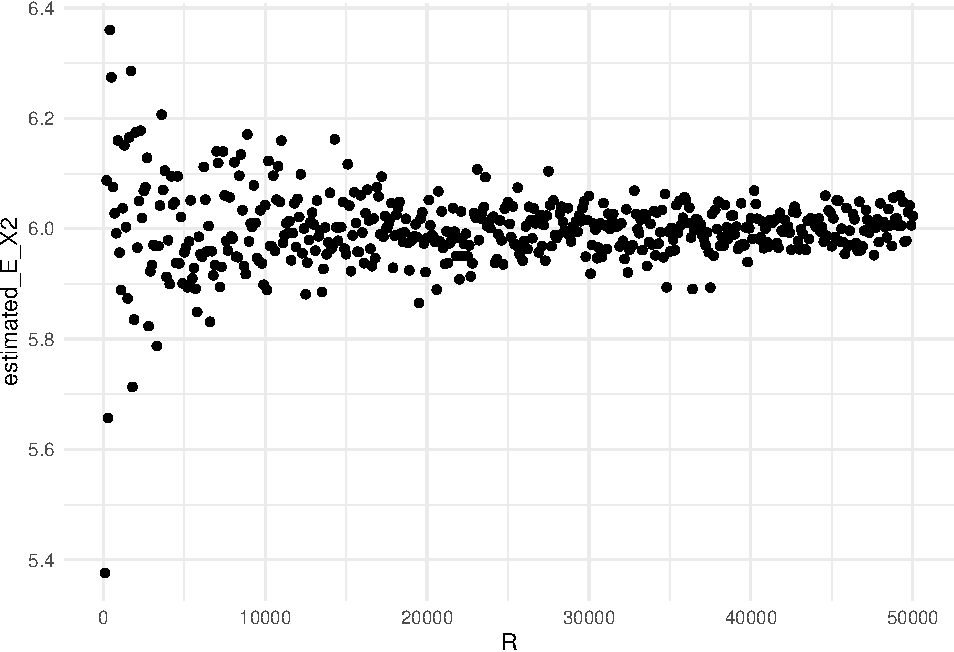
\includegraphics{Homework1_files/figure-latex/unnamed-chunk-22-1.pdf}

\end{document}
